\chapter{Introduction}
\section{Project Aims}

The aim of this project is to build a attendance monitoring system than is able to track attendance while 
The main evaluation criteria

\section{Related Works} 



\subsection{Subsection of a Section}
\subsubsection{Subsection of a Subsection}

Example of double quotes ``word''. 

Example of citation \citep{altschul1997gapped}.  

Example of multiple citations \citep{altschul1997gapped,baker2007novel}. 

\newglossaryentry{maths}{name={maths}, description={What mathemeticians do.}}
\glsadd{maths}
Example of italic text - {\it Escherichia}, {\it Salmonella}, and {\it Shigella} spp. 

Example of hyperlink \url{http://www.wikibooks.org}. 

Another example of hyperlink \href{http://www.wikibooks.org}{Wikibooks home}. 

LaTeX{} has a special way to embed maths symbols and notations. Here are some of them. Also observe how a bullet list is made.

\begin{itemize}\itemsep0pt \parskip0pt \parsep0pt
\item greater than $\ge$
\item less than $\le$
\item percent sign \%
\item multiply $N\times N$
\item inline equation $M = N(N-1)/2$
\end{itemize}

Example of a mathematical formula:
\begin{equation}
  ADD = \sum_{i=1}^{M}|<D(n+1,i)>-<D(n,i)>|
  \label{add}
\end{equation}

Example of a figure.
\begin{figure}[ht!]
\begin{center}
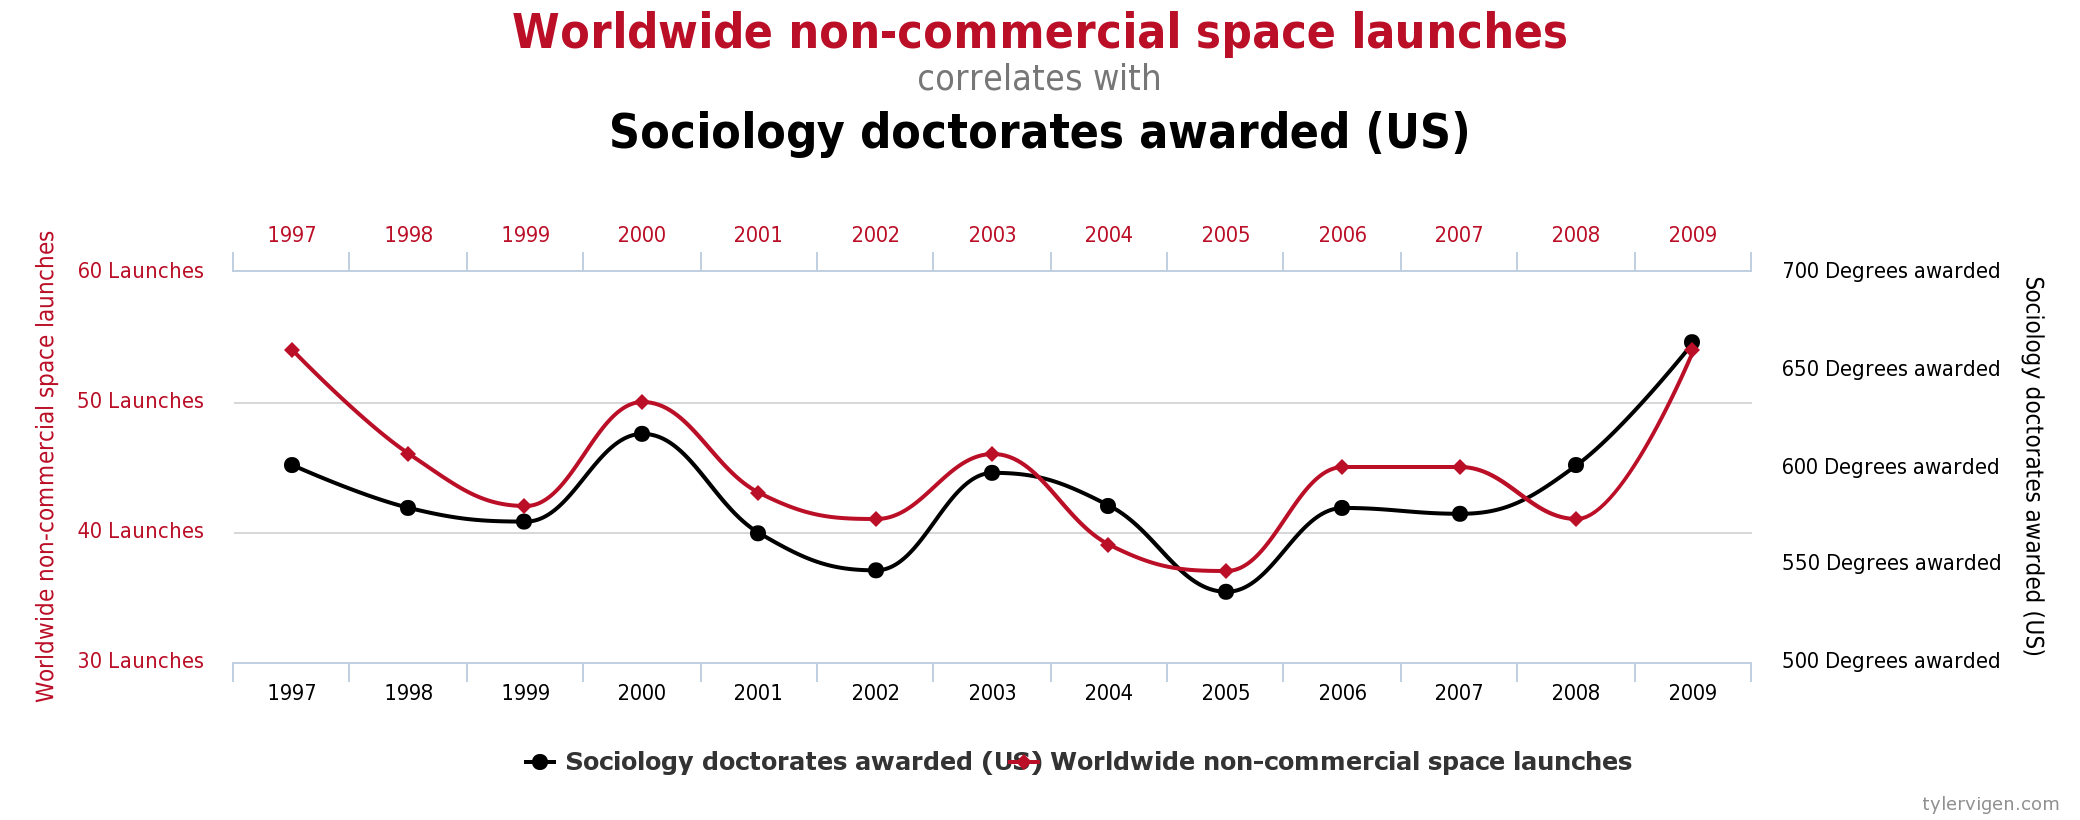
\includegraphics[scale=0.2]{chapter1/images/example_graph.png}
\end{center}
\caption{An example graph}
\label{graph1}
\end{figure}

Example of a table and here is the reference to Table \ref{table_genomes}. 

\begin{table}
\begin{center}
\begin{tabular}{|l|c|c|c|}
\hline
{\sc Organism}  &  {\sc Accession no.}  & {\sc Genome size} (bp)  & {\sc No. CDS} \\
\hline
{\it Mesorhizobium loti}          & NC\_002678 & 7036071 & 6743 \\
\hline
{\it Sinorhizobium meliloti}      & NC\_003047 & 3654135 & 3359 \\
\hline
{\it Bradyrhizobium japonicum}    & NC\_004463 & 9105828 & 8317 \\
\hline
{\it Rhodopseudomonas palustris}  & NC\_005296 & 5459213 & 4813 \\
\hline
{\it Bartonella quintana}         & NC\_005955 & 1581384 & 1142 \\
\hline
{\it Bartonella henselae}         & NC\_005956 & 1931047 & 1488 \\
\hline
{\it Rickettsia typhi}            & NC\_006142 & 1111496 & 837 \\
\hline
{\it Beijerinckia indica}         & NC\_010581 & 4170153 & 3569 \\
\hline
\end{tabular}
\end{center}
\caption{Whole-genome sequences used in this study}
\label{table_genomes}
\end{table}

With the currently existing projects and literature in this field
